\subsection{Socket server}
Kernen af CentralServer’s funktionalitet er en socket server, som lytter efter og accepterer forbindelser fra klienter. Når serveren modtager en ny forbindelse fra en klient bliver der oprettet en ny instans af ClientControl, som håndterer kommunikationen med klienten. Denne instans af ClientControl bliver sendt til MainControl, som overtager alle referencer til klienten. SocketServer kender derfor ikke til åbne forbindelser.\\

Figur \ref{fig:CSSocketServer} viser UML-digram for SocketServer.


\begin{figure}[H]
    \centering
    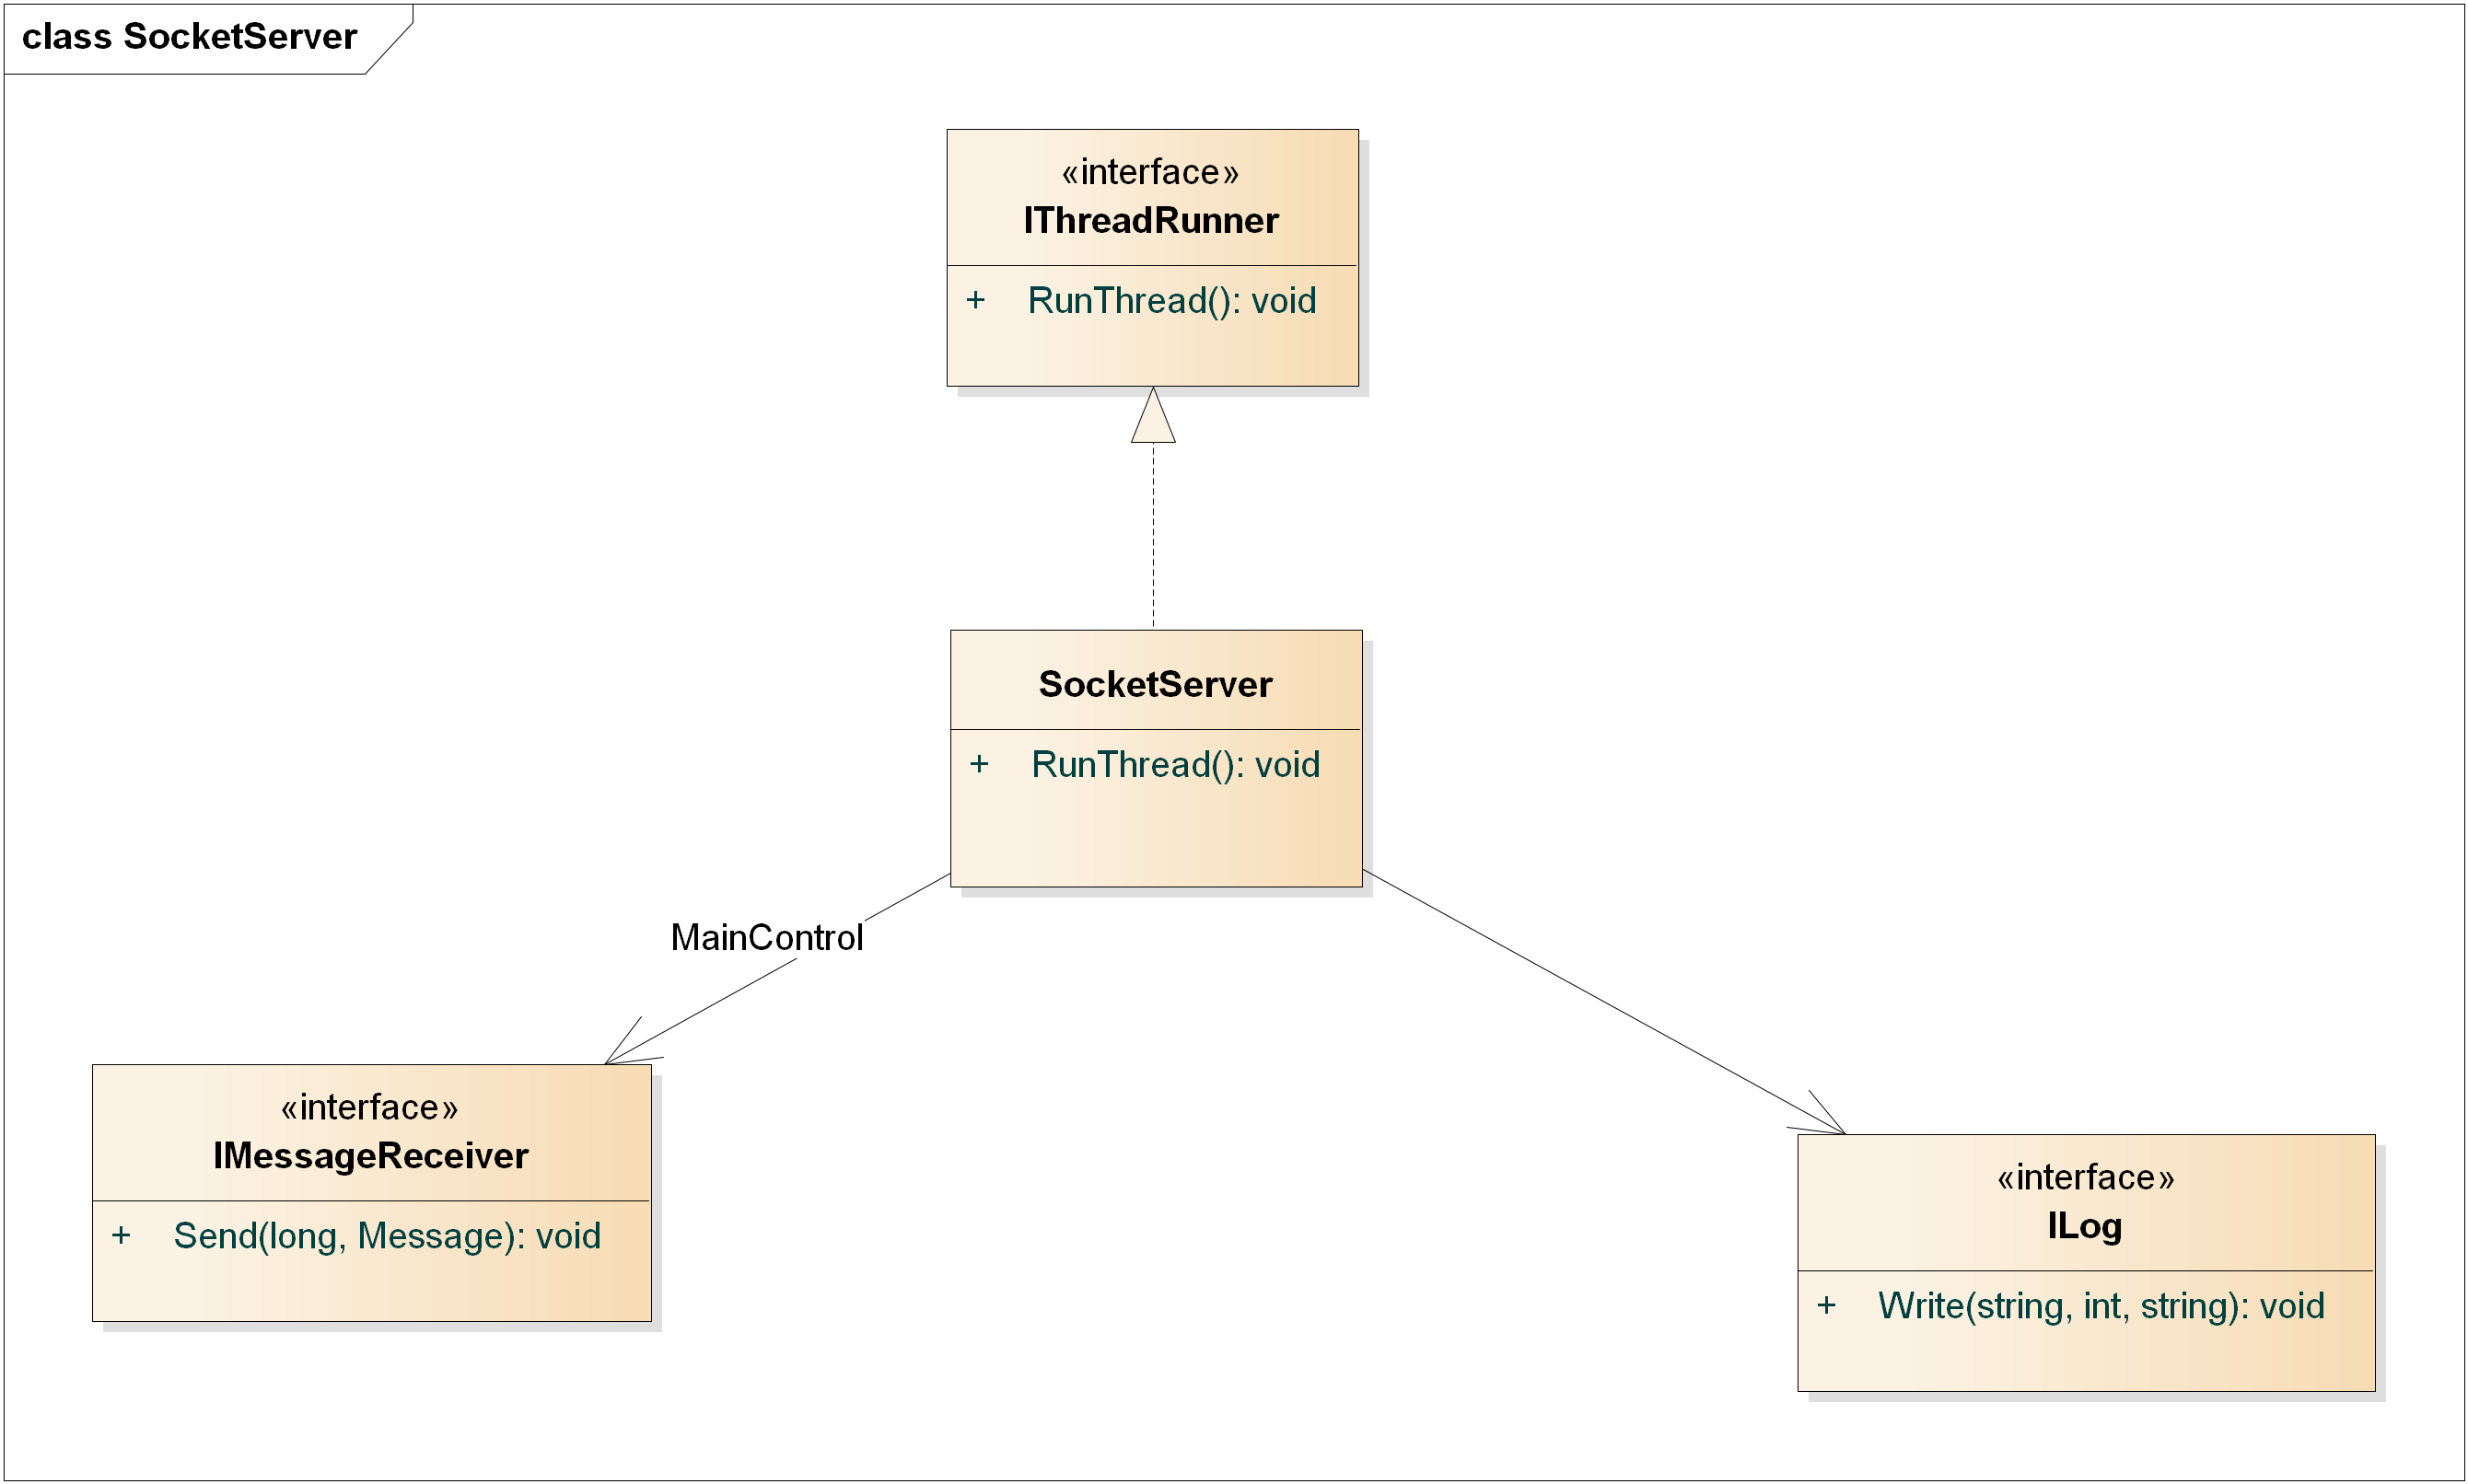
\includegraphics[width=1\textwidth]{Systemdesign/CentralServer/Images/SocketServer.png}
    \caption{UML-diagram for SocketServer}
    \label{fig:CSSocketServer}
\end{figure}


\textbf{Accept af forbindelser}\\
På Figur \ref{fig:CSAcceptConnections} ses, hvordan SocketServer accepterer indkommende forbindelser fra nye klienter og sender klienten videre til MainControl.

\begin{itemize}
  \item SocketServer opretter en ny instans af SocketConnection.
  \item SocketServer opretter en ny instans af ClientControl, som får SocketConnection med som parameter.
  \item ClientControl binder på følgende events fra SocketConnection: OnDataRecieved og OnDisconnect.
  \item SocketServer sender en E\_START\_SESSION besked til MainControl, hvor den nye ClientControl gives med som parameter.
  \item MainControl modtager beskeden, og registrerer den nye klient i SessionControl. MainControl får et sessions ID tilbage.
  \item MainControl sender en E\_WELCOME til ClientControl med sessions ID'et.
  \item ClientControl kalder StartRecieving() på SocketConnection for at begynde at modtage data herfra.
\end{itemize}

\begin{figure}[H]
    \centering
    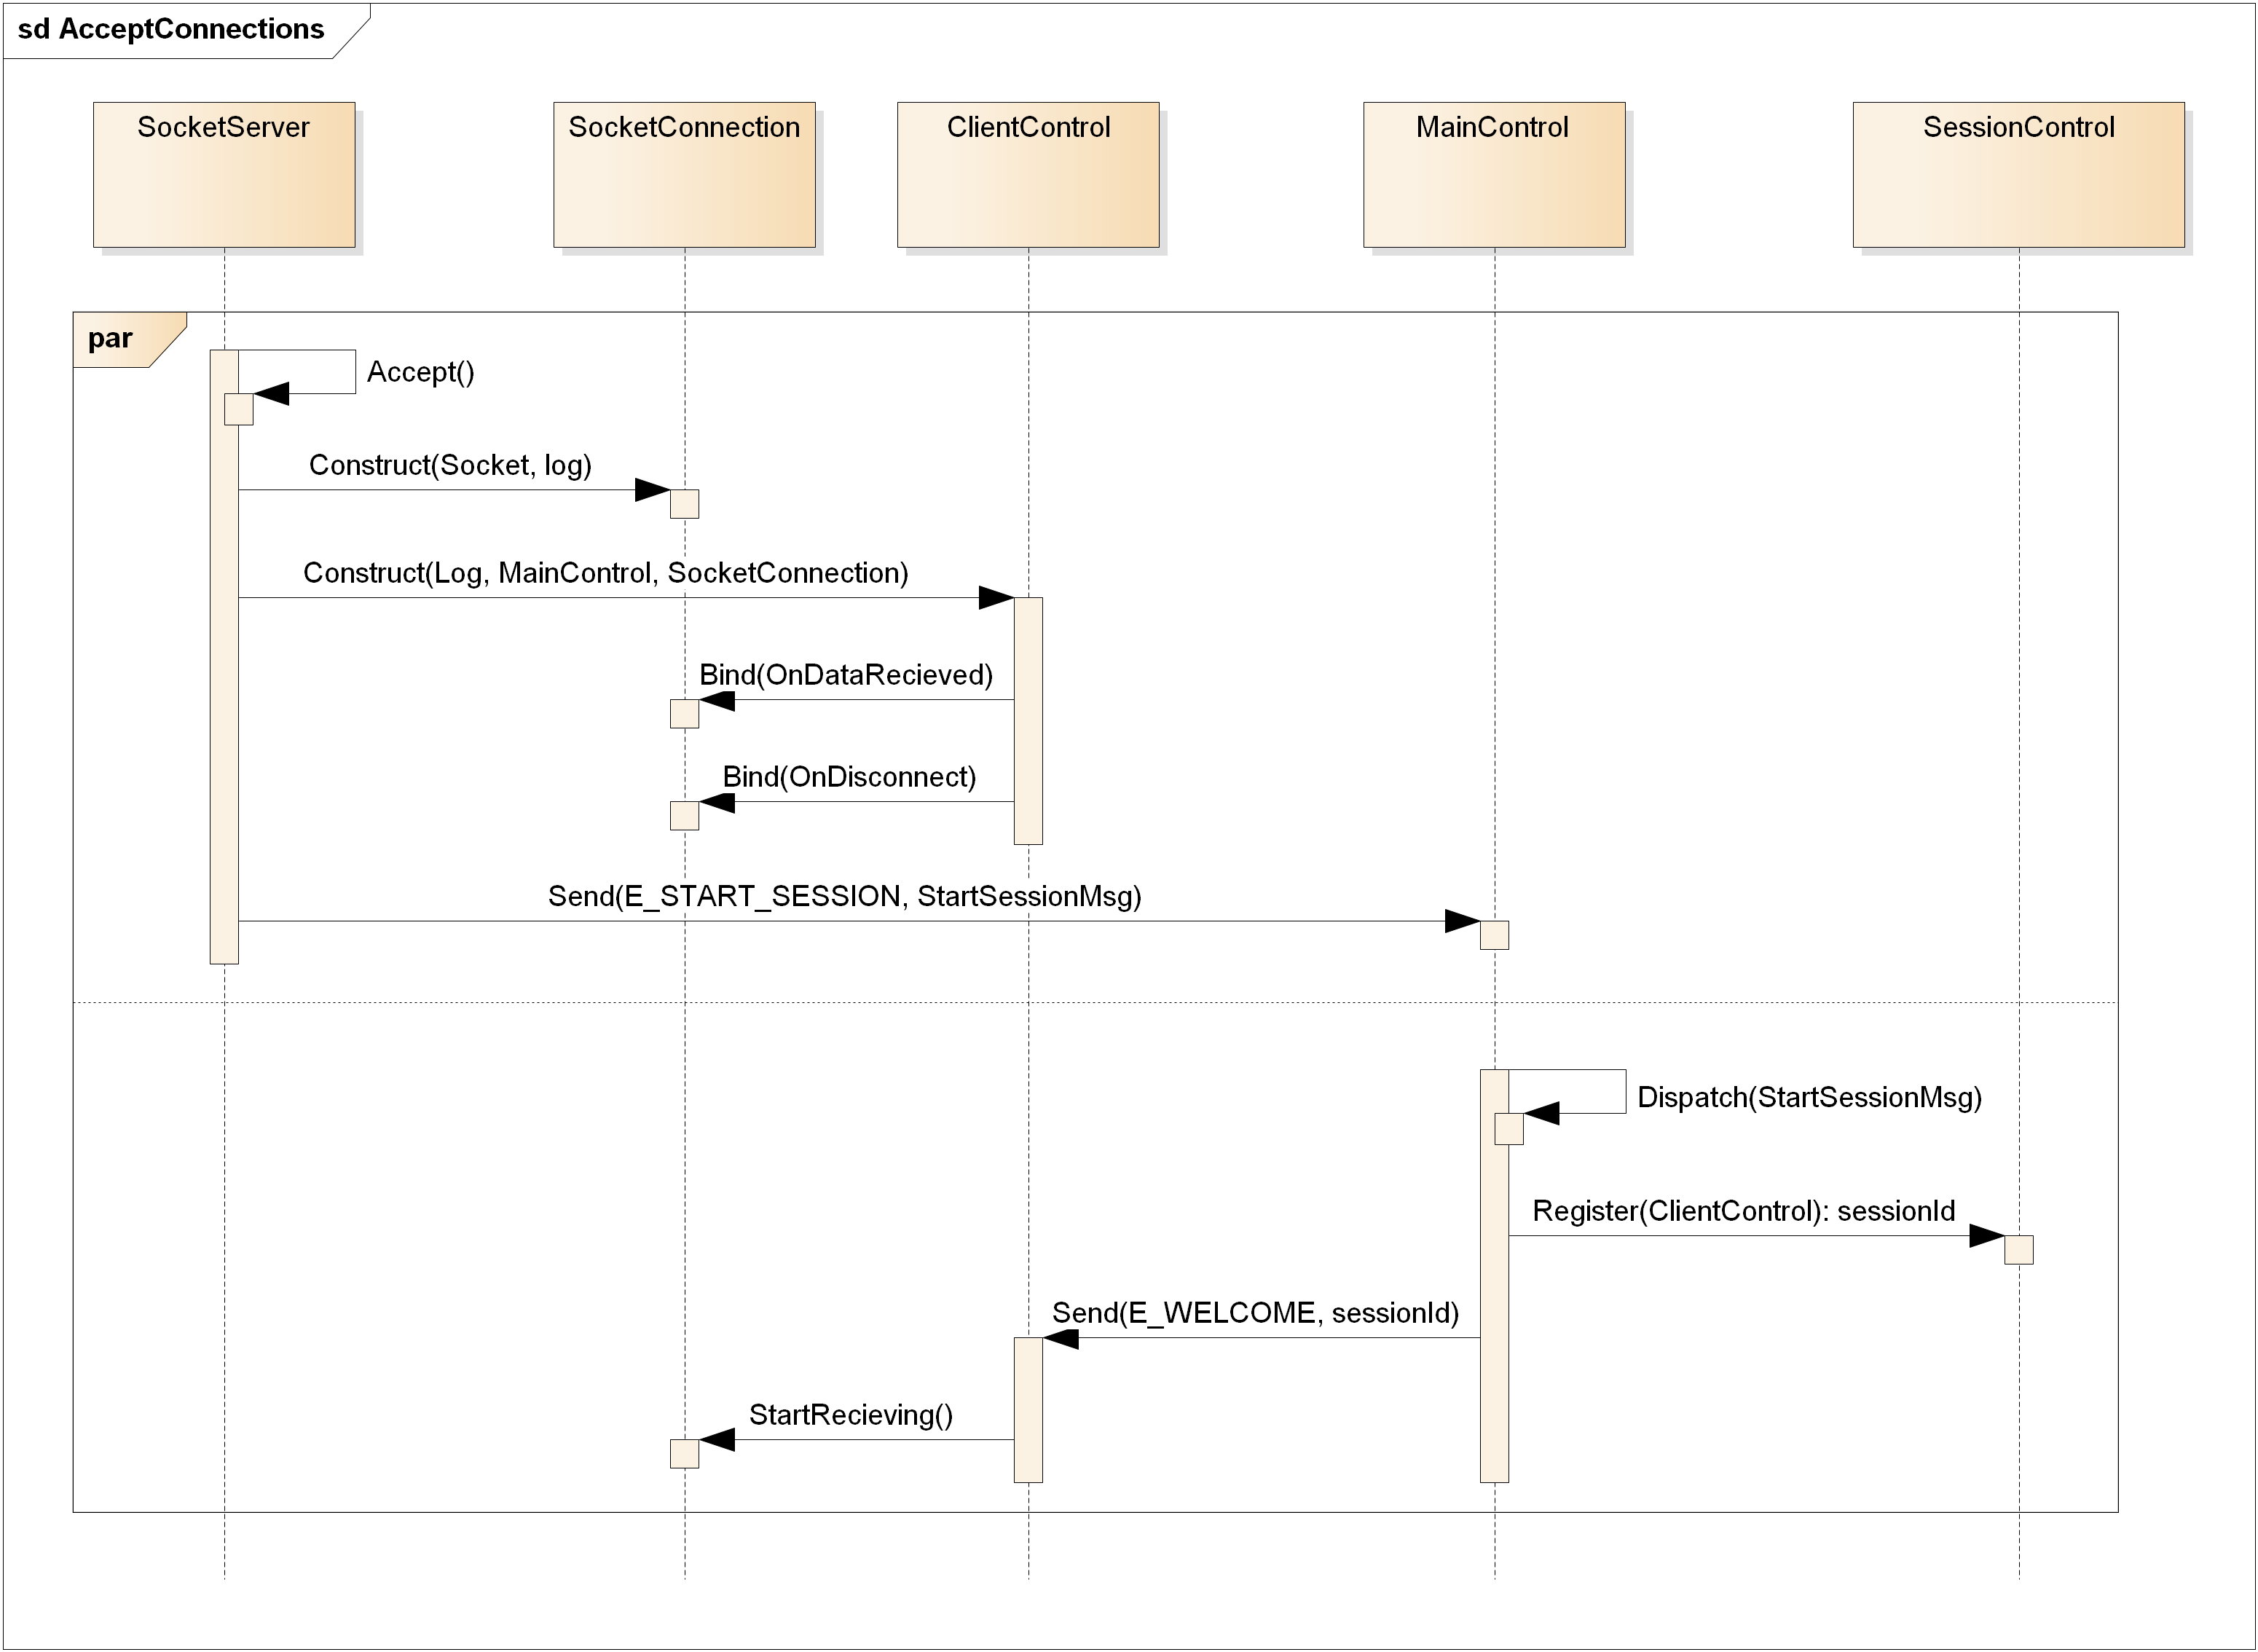
\includegraphics[width=1\textwidth]{Systemdesign/CentralServer/Images/AcceptConnections.png}
    \caption{Sekvensdiagrammet viser accept-processen for nye klienter}
    \label{fig:CSAcceptConnections}
\end{figure}

\textbf{Modtagelse af data}\\
På Figur \ref{fig:CSReadData} ses, hvordan data modtages fra klienten, som parses og sendes til MainControl.

\begin{itemize}
  \item SocketConnection læser data fra en socket.
  \item SocketConnection kalder HandleDataRecieved på ClientControl med den rå data streng.
  \item ClientControl kalder AddData() på Protocol klassen med den rå data streng.
  \item ClientControl kalder herefter GetCommands() på Protocol klassen, som returnerer en liste med alle komplette kommandoer, der er modtaget.
  \item ClientControl sender herefter en E\_COMMAND\_RECEIVED besked til MainControl.
\end{itemize}

\begin{figure}[H]
    \centering
    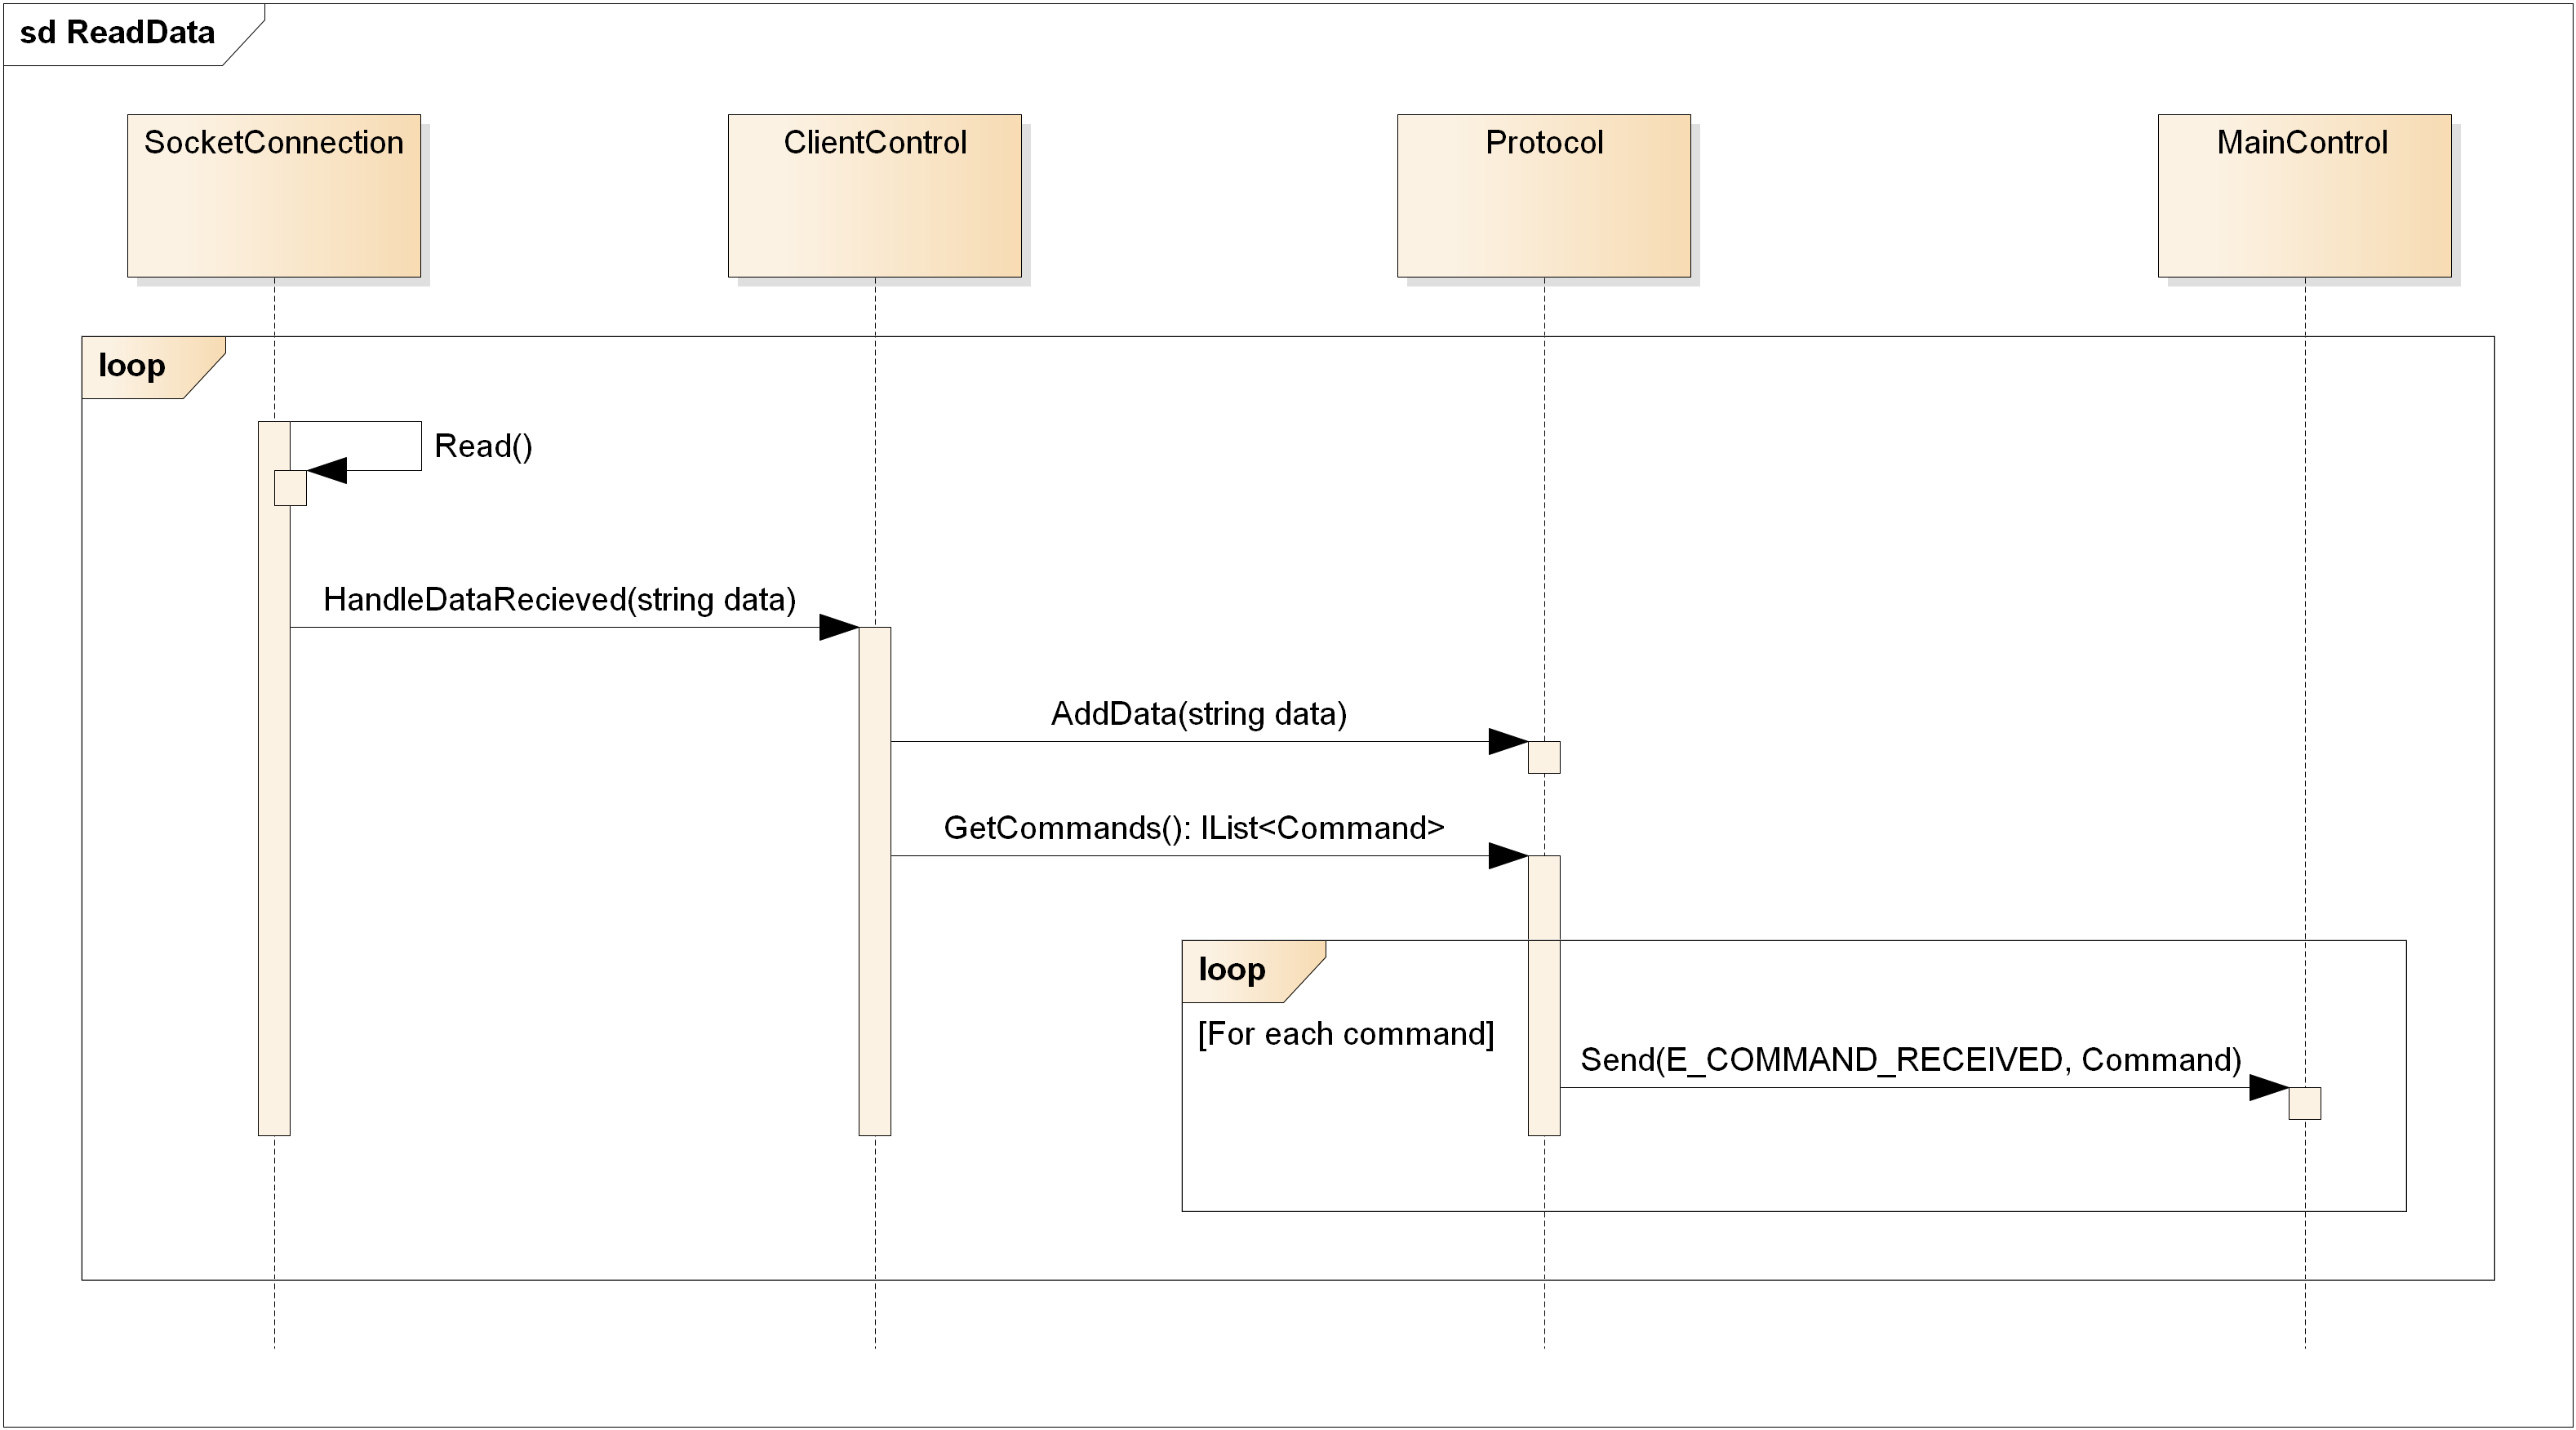
\includegraphics[width=1\textwidth]{Systemdesign/CentralServer/Images/ReadData.png}
    \caption{Sekvensdiagrammet viser hvordan der modtages data fra klienter}
    \label{fig:CSReadData}
\end{figure}

\textbf{Lukning af forbindelser}\\
På Figur \ref{fig:CSCloseConnection} ses, hvordan CentralServer håndterer, at klienter lukker forbindelsen til serveren.

\begin{itemize}
  \item SocketConnection registrerer, at klienten har lukket forbindelsen til serveren.
  \item SocketConnection kalder HandleConnectionClosed på ClientControl.
  \item ClientControl sender en E\_STOP\_SESSION til MainControl med sessions ID som parameter.
  \item MainControl kalder UnregisterSession() på SessionControl.
\end{itemize}

\begin{figure}[H]
    \centering
    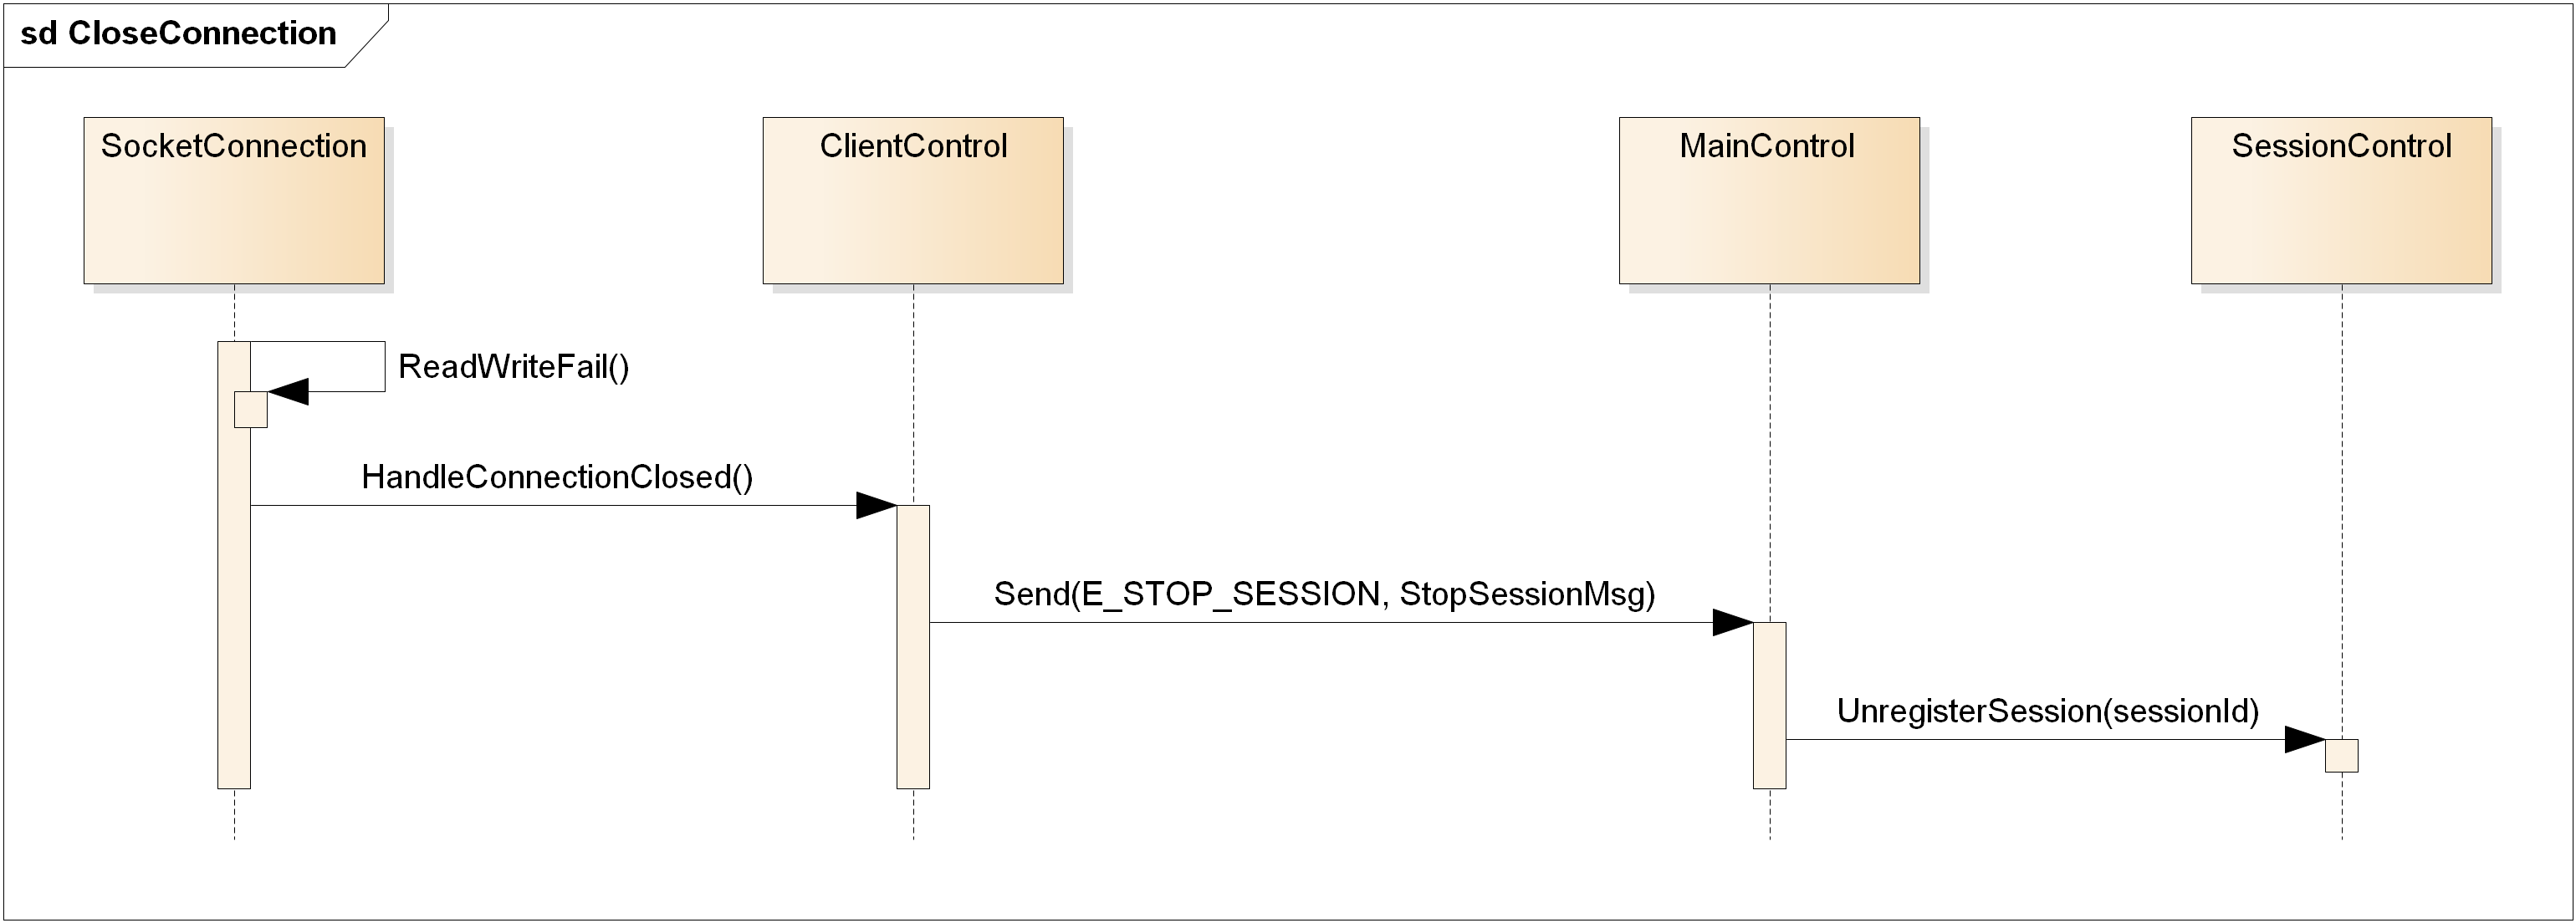
\includegraphics[width=1\textwidth]{Systemdesign/CentralServer/Images/CloseConnection.png}
    \caption{Sekvensdiagrammet viser hvordan CentralServer håndterer, at klienter lukker forbindelsen til serveren}
    \label{fig:CSCloseConnection}
\end{figure}
